\documentclass[10.5pt,scale=1.0,t,aspectratio=169,hyperref={pdfpagelabels=false}]{beamer}
\usepackage{lipsum}
\usepackage{color}
\usepackage{amsfonts}
\usepackage{amsmath,mathtools}
\usepackage{mathrsfs}
\usepackage{array}
\usepackage{algorithm}
\usepackage{hyperref}
\usepackage[spanish,es-nodecimaldot]{babel}
\usepackage[utf8]{inputenc}
\usepackage{graphicx}
\usepackage{multicol}
\usepackage{multirow}
\usepackage{enumitem}
\usepackage[document]{ragged2e}
\usepackage[absolute,overlay]{textpos}
\textblockorigin{0mm}{0mm} 
\usefonttheme[onlymath]{serif}
\usepackage{verbatim}
\usepackage{cite}
\usepackage{multicol}
\usepackage{siunitx}




\newenvironment{conditions}[1][where:]
{#1 \begin{tabular}[t]{>{$}l<{$} @{${}={}$} l}}
	{\end{tabular}\\[\belowdisplayskip]}


\newcolumntype{L}{>{$}l<{$}} % math-mode version of "l" column type


\newcounter{saveenumi}
\newcommand{\seti}{\setcounter{saveenumi}{\value{enumi}}}
\newcommand{\conti}{\setcounter{enumi}{\value{saveenumi}}}

\setbeamertemplate{bibliography item}{\insertbiblabel}


\hypersetup{colorlinks=true,
	linkcolor=blue,
	linktoc=all,				
	citecolor=blue,
	urlcolor=red,
	pdftitle={ELECTRONICA DIGITAL},
	pdfauthor={Santiago Rúa Pérez},
	pdfcreator={Santiago Rúa Pérez}}


\definecolor{GreenDark}{rgb}{0.0, 0.60, 0.0}
\definecolor{RedDark}{rgb}{183, 0.0, 0.0}
\definecolor{BlueDark}{rgb}{0.0, 0.0, 167}
\definecolor{BlueLight}{rgb}{0.2, 0.451, 0.517}


\graphicspath{{imag/}}

\newcommand{\Ho}{$H_{0}$}
\newcommand{\Ha}{$H_{a}$}
\newcommand{\Nota}{{\bf Nota: }}
\newcolumntype{P}[1]{>{\centering\arraybackslash}p{#1}}
\newcolumntype{M}[1]{>{\centering\arraybackslash}m{#1}}

\newcommand{\less}{<}
\newcommand{\greater}{>}


\setlength{\parindent}{1em}
\setlength{\parskip}{.6em}
\renewcommand{\baselinestretch}{.9}

%%%%    C environment    ---------------- %%%%%%%%%%%%%%%.
\usepackage{listings}
\usepackage{xcolor}
\definecolor{mGreen}{rgb}{0,0.6,0}
\definecolor{mGray}{rgb}{0.5,0.5,0.5}
\definecolor{mPurple}{rgb}{0.58,0,0.82}
\definecolor{backgroundColour}{rgb}{0.95,0.95,0.92}

\lstdefinestyle{CStyle}{
	backgroundcolor=\color{backgroundColour},   
	commentstyle=\color{mGreen},
	keywordstyle=\color{magenta},
	numberstyle=\tiny\color{mGray},
	stringstyle=\color{mPurple},
	basicstyle=\tiny,
	breakatwhitespace=false,         
	breaklines=true,                 
	captionpos=b,                    
	keepspaces=true,                 
	numbers=left,                    
	numbersep=5pt,                  
	showspaces=false,                
	showstringspaces=false,
	showtabs=false,                  
	tabsize=2,
	language=C
}


%%--------------------------------------------------------------------------

\title{Electrónica Digital II}   
\author{Santiago Rúa Pérez, PhD.} 
\date{\today} 

\setlength{\TPHorizModule}{\textwidth}
\setlength{\TPVertModule}{\textwidth}

\newcommand{\btVFill}{\vskip0pt plus 1filll}


\setbeamertemplate{sidebar right}{}
\setbeamertemplate{footline}
{
	\leavevmode%
	\hbox{%
		\begin{beamercolorbox}[wd=.333333\paperwidth,ht=2.25ex,dp=1ex,center]{author in head/foot}%
			\usebeamerfont{author in head/foot}\insertshortauthor
		\end{beamercolorbox}%
		\begin{beamercolorbox}[wd=.333333\paperwidth,ht=2.25ex,dp=1ex,center]{title in head/foot}%
			\usebeamerfont{title in head/foot}\insertshorttitle
	\end{beamercolorbox}}%
	\vskip0pt%
}
\makeatother

\begin{document}
	%%%%%%%%%%%%%%%%%% FRAME %%%%%%%%%%%%%%%%%%%%%%%%%%
	\begin{frame}
		\titlepage
	\end{frame}




	%%%%%%%%%%%%%%%%% FRAME START %%%%%%%%%%%%%%%%%%%%%%%%%%
	\frame{
		%\frametitle{}
		\begin{center}
			\LARGE \textcolor{blue}{GENERAL PURPOSE INPUT-OUTPUT GPIO}
		\end{center}
		
	}
	
	%%%%%%%%%%%%%%%%% FRAME %%%%%%%%%%%%%%%%%%%%%%%%%%

%%%%%%%%%%%%%%%%% FRAME %%%%%%%%%%%%%%%%%%%%%%%%%%
\begin{frame}
\frametitle{Objetivos}
\begin{itemize}
\item Entender como utilizar los puertos de propósitos generales de entrada y salida. 
\item Entender los registros de acceso a los puertos de propósito generales.
\item Comprender el funcionamiento del LCD y teclado matricial.
\end{itemize}
\end{frame}
%%%%%%%%%%%%%%%%% FRAME %%%%%%%%%%%%%%%%%%%%%%%%%%
\begin{frame}
	\frametitle{Panorama general}
	\begin{itemize}
		\item Cómo podemos hacer para encender un led que dependa de la respuesta de un suiche?
		\item Entender como es la interfaz de los circuitos.
		\item Periféricos GPIO.
		\item LCD y teclado matricial. 
	\end{itemize}
\end{frame}

%%%%%%%%%%%%%%%%% FRAME %%%%%%%%%%%%%%%%%%%%%%%%%%
\begin{frame}
	\frametitle{Conceptos básicos}
	\begin{figure}
		\centering
		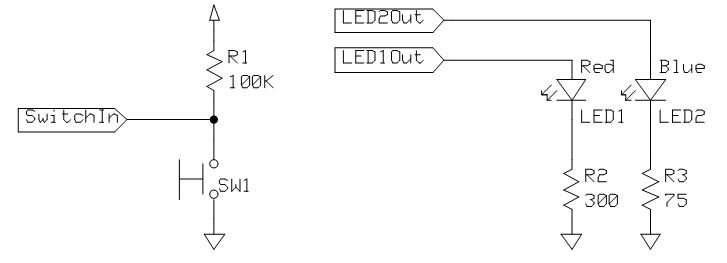
\includegraphics[scale=0.4]{01_BasicConcept}
	\end{figure}
	\begin{itemize}
		\item Fin: encender LED1 o LED2 de acuerdo al estado del suiche SW1.
		\item GPIO: General-purpose input and output
		\begin{itemize}
			\item Entrada: el programa puede determinar si la señal de entrada es 1 o 0.
			\item Salida: el programa pone un 1 o 0 en el pin. 
		\end{itemize}
		\item Pueden ser utilizado como interfaz con dispositivos externos.
		\begin{itemize}
			\item Entrada: suiche
			\item Salida: LEDs.
		\end{itemize}
	\end{itemize}
\end{frame}
%%%%%%%%%%%%%%%%% FRAME %%%%%%%%%%%%%%%%%%%%%%%%%%
\begin{frame}
	\frametitle{Entradas: Qué es un cero y qué es un uno?}
	\begin{columns}
		\column{0.4\linewidth}
		\begin{itemize}
			\item El valor de la entrada de señal es determinada por el voltaje.
			\item Los límites de voltaje dependerán de la alimentación del sistema. Es una medida relativa.
			\item Alimentar con un valor mayor al de alimentación $V_{DD}$ o inferior a GND puede generar un daño en el dispositivo. 
		\end{itemize}
		\column{0.6\linewidth}
		\begin{figure}
			\centering
			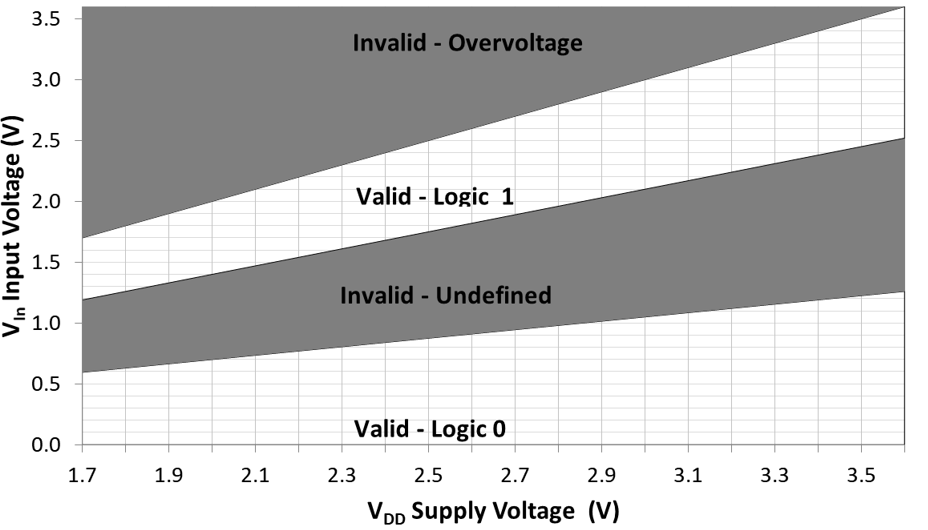
\includegraphics[scale=0.35]{02_ThresholdVoltage}
		\end{figure}
	\end{columns}
\end{frame}
%%%%%%%%%%%%%%%%% FRAME %%%%%%%%%%%%%%%%%%%%%%%%%%
\begin{frame}
	\frametitle{Salida: Qué es un cero y qué es un uno?}
	\begin{columns}
		\column{0.5\linewidth}
		\begin{itemize}
			\item Salida de voltajes nominales
			\begin{itemize}
				\item 1: $V_{DD}$-\SI{0.5}{\volt} to $V_{DD}$
				\item 0: 0 to \SI{0.5}{\volt}.
			\end{itemize}
			\item Nota: La salida de voltaje dependerá de la corriente demandada por el circuito.
			\begin{itemize}
				\item Se necesita considerar la resistencia entre la fuente y el drenaje en el transistor. 
				\item Los valores anteriores solo se especifican para corrientes de menos de \SI{5}{\milli\ampere} (\SI{18}{\milli\ampere} para pines de alta corriente ) y $V_{DD}$ mayor a \SI{2.7}{\volt}
			\end{itemize}
		\end{itemize}
		\column{0.5\linewidth}
		\begin{figure}
			\centering
			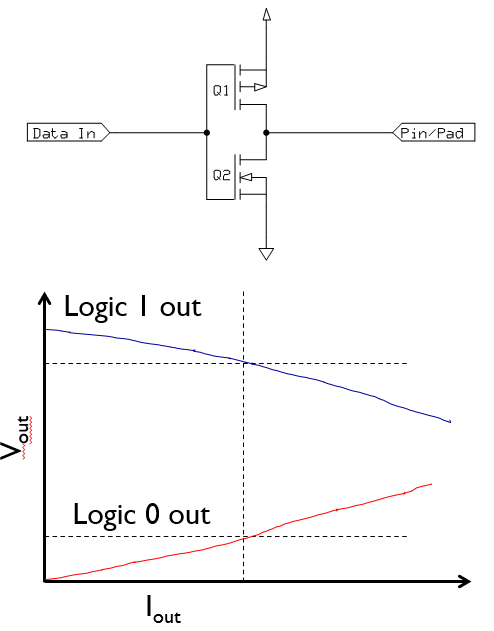
\includegraphics[scale=0.35]{03_OutputDrain}
		\end{figure}
	\end{columns}
\end{frame}
%%%%%%%%%%%%%%%%% FRAME %%%%%%%%%%%%%%%%%%%%%%%%%%
\begin{frame}
	\frametitle{Ejemplo de salida: Conectar un LED}
	\begin{columns}
		\column{0.7\linewidth}
		\begin{itemize}
			\item Limitar la corriente a un nivel seguro para el LED y el pin del microcontrolador.
			\item Usar resistencia limitadora de corriente. 
			\begin{itemize}
				\item $R = (V_{DD}-V_{LED})/I_{LED}$
			\end{itemize}
			\item Seleccionar la corriente del LED alrededor de \SI{4}{\milli\ampere}
			\item El voltaje en el led dependerá de su color.
			\begin{itemize}
				\item Rojo: $\approx$\SI{1.8}{\volt}
				\item Azul: $\approx$\SI{2.7}{\volt}
			\end{itemize}
			\item Resolver R dado que la alimentacion es alrededor de \SI{3}{\volt}.
			\begin{itemize}
				\item Rojo: \SI{300}{\Omega}
				\item Azul: \SI{75}{\Omega}
			\end{itemize}
		\end{itemize}
	
		\column{0.3\linewidth}
		\begin{figure}
			\centering
			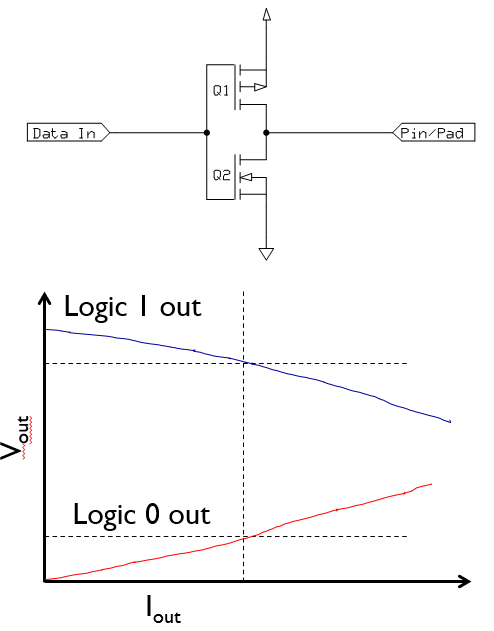
\includegraphics[scale=0.35]{03_OutputDrain}
		\end{figure}
	\end{columns}
\end{frame}
%%%%%%%%%%%%%%%%% FRAME %%%%%%%%%%%%%%%%%%%%%%%%%%
\begin{frame}
	\frametitle{Hardware del GPIO}
	\begin{columns}
		\column{0.4\linewidth}
		\begin{itemize}
			\item Se tiene desde el puerto A al E.
			\item No todos los bits de los puertos estan disponibles.
			\item La cantidad dependerá del footprint del chip. 
		\end{itemize}
		
		\column{0.6\linewidth}
		\begin{figure}
			\centering
			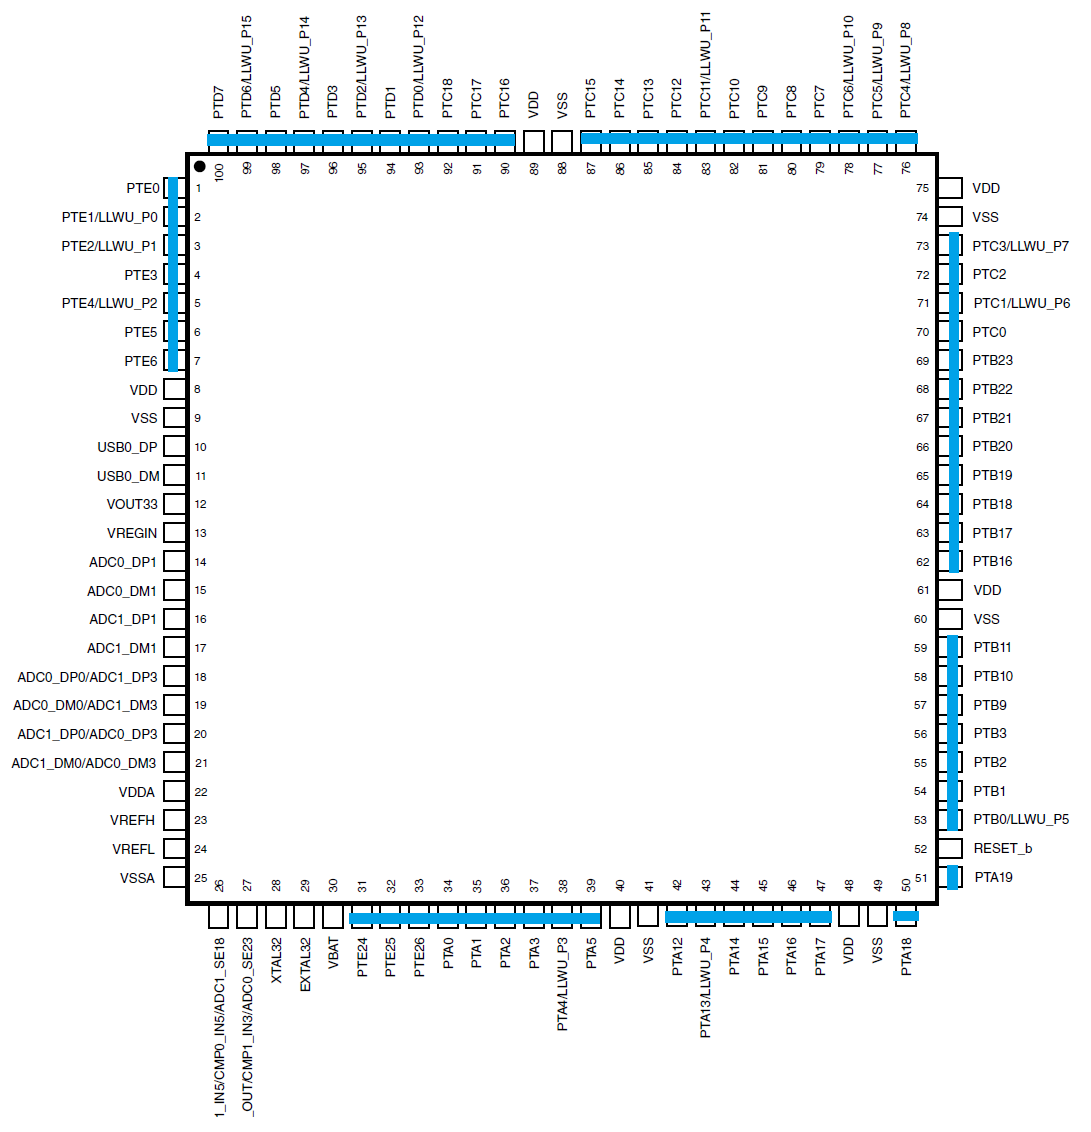
\includegraphics[scale=0.35]{04_GPIOPorts}
		\end{figure}
	\end{columns}
\end{frame}
%%%%%%%%%%%%%%%%% FRAME %%%%%%%%%%%%%%%%%%%%%%%%%%
\begin{frame}
	\frametitle{Hardware del GPIO - FRDM}
	\begin{columns}
		\column{0.4\linewidth}
		\begin{itemize}
			\item No todos los pins estan accesibles.  
			\item El led RGB esta conectado a 3 puertos.
			\begin{itemize}
				\item Rojo: PTB22
				\item Azul: PTB21
				\item Verde: PTE26
			\end{itemize}
			\item Los pulsadores también. 
			\begin{itemize}
				\item SW2: PTC6
				\item SW3: PTA4
			\end{itemize}
		\end{itemize}
		
		\column{0.6\linewidth}
		\begin{figure}
			\centering
			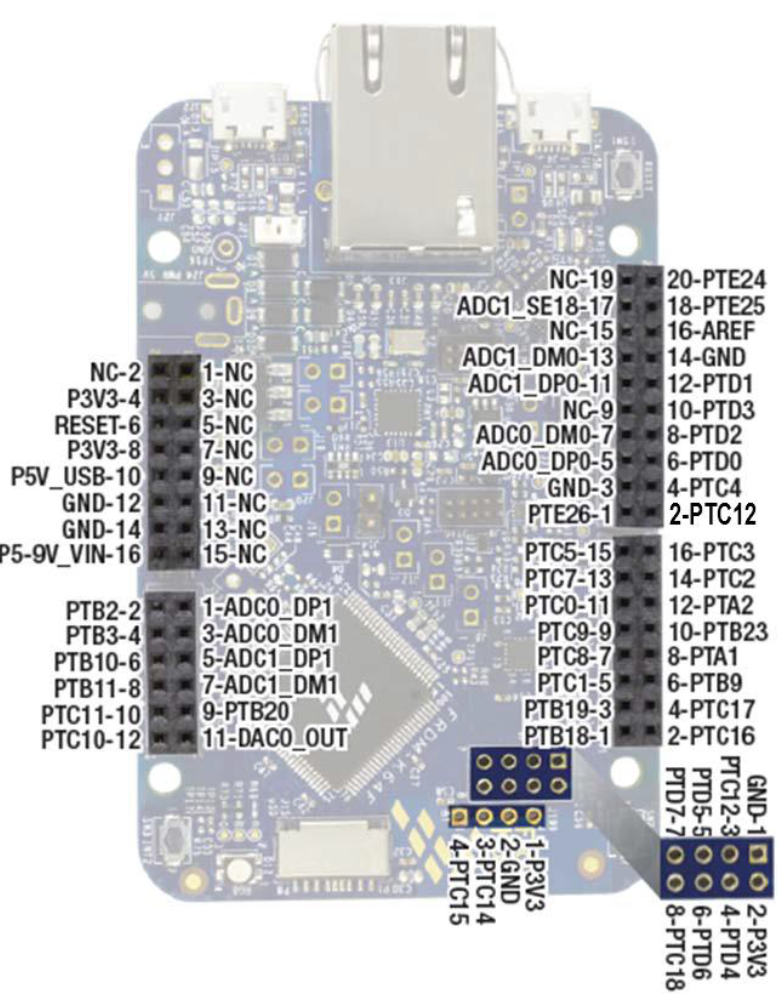
\includegraphics[scale=0.4]{05_GPIOPortsFRDM}
		\end{figure}
	\end{columns}
\end{frame}
%%%%%%%%%%%%%%%%% FRAME %%%%%%%%%%%%%%%%%%%%%%%%%%
\begin{frame}
	\frametitle{Pines Compartidos}
		\begin{figure}
			\centering
			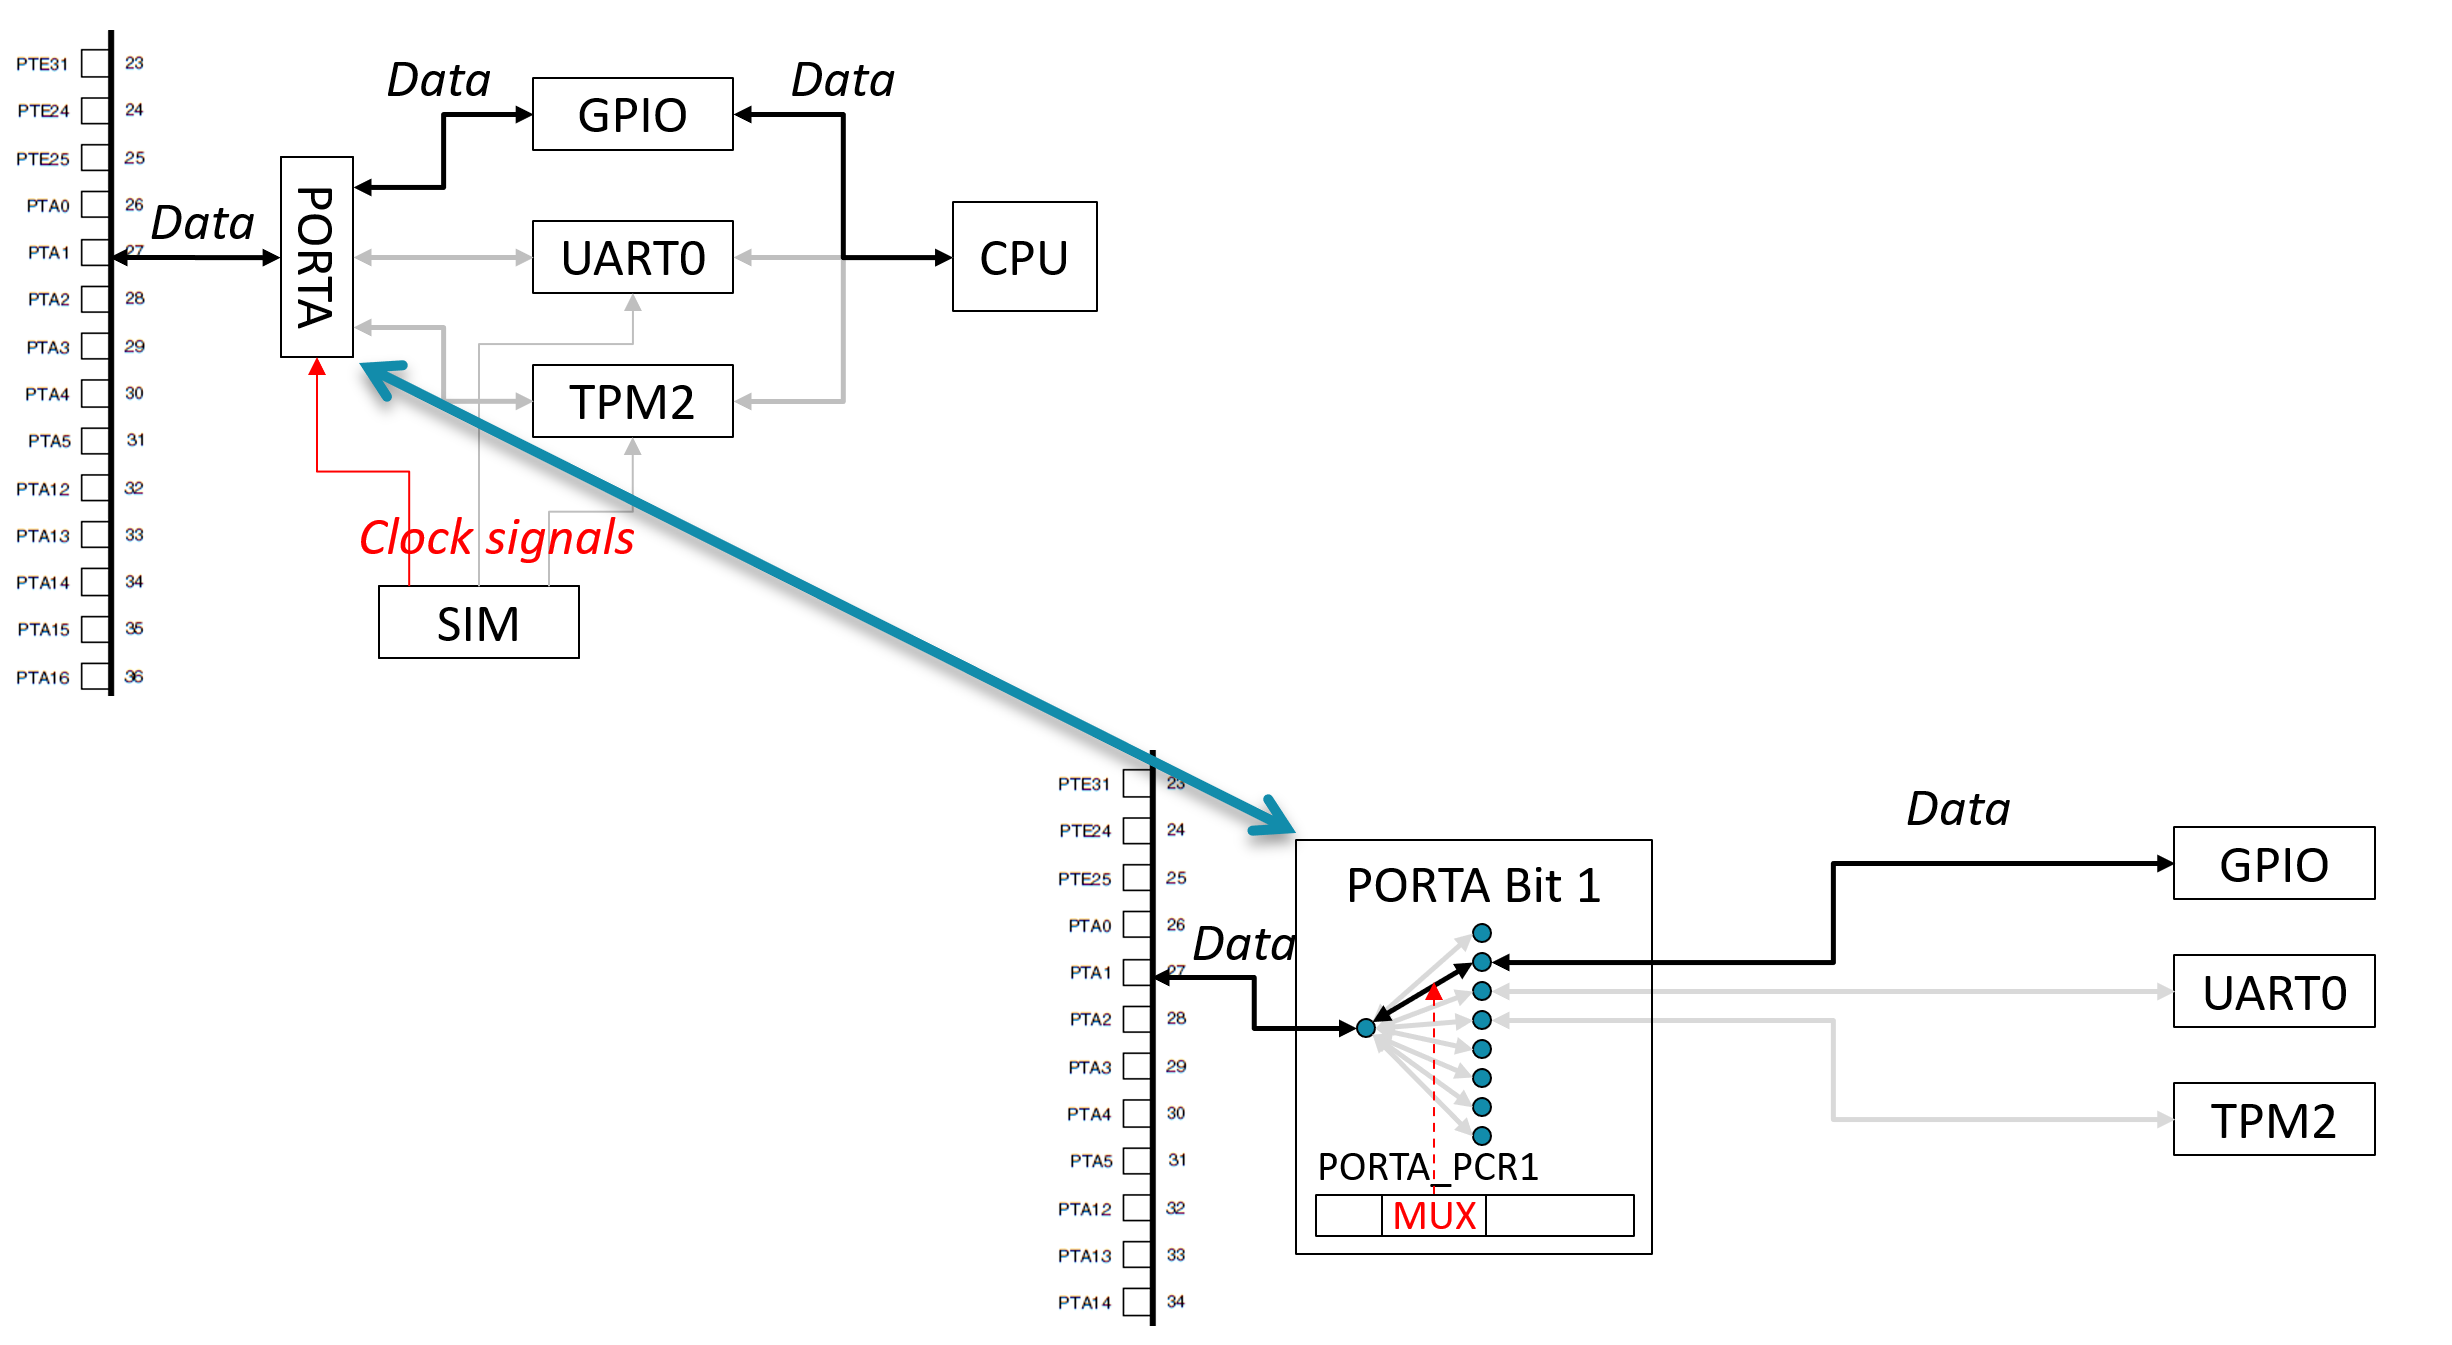
\includegraphics[scale=0.3]{06_GPIOShared}
		\end{figure}
\end{frame}
%%%%%%%%%%%%%%%%% FRAME %%%%%%%%%%%%%%%%%%%%%%%%%%
\begin{frame}
	\frametitle{Circuito del GPIO}
	\begin{figure}
		\centering
		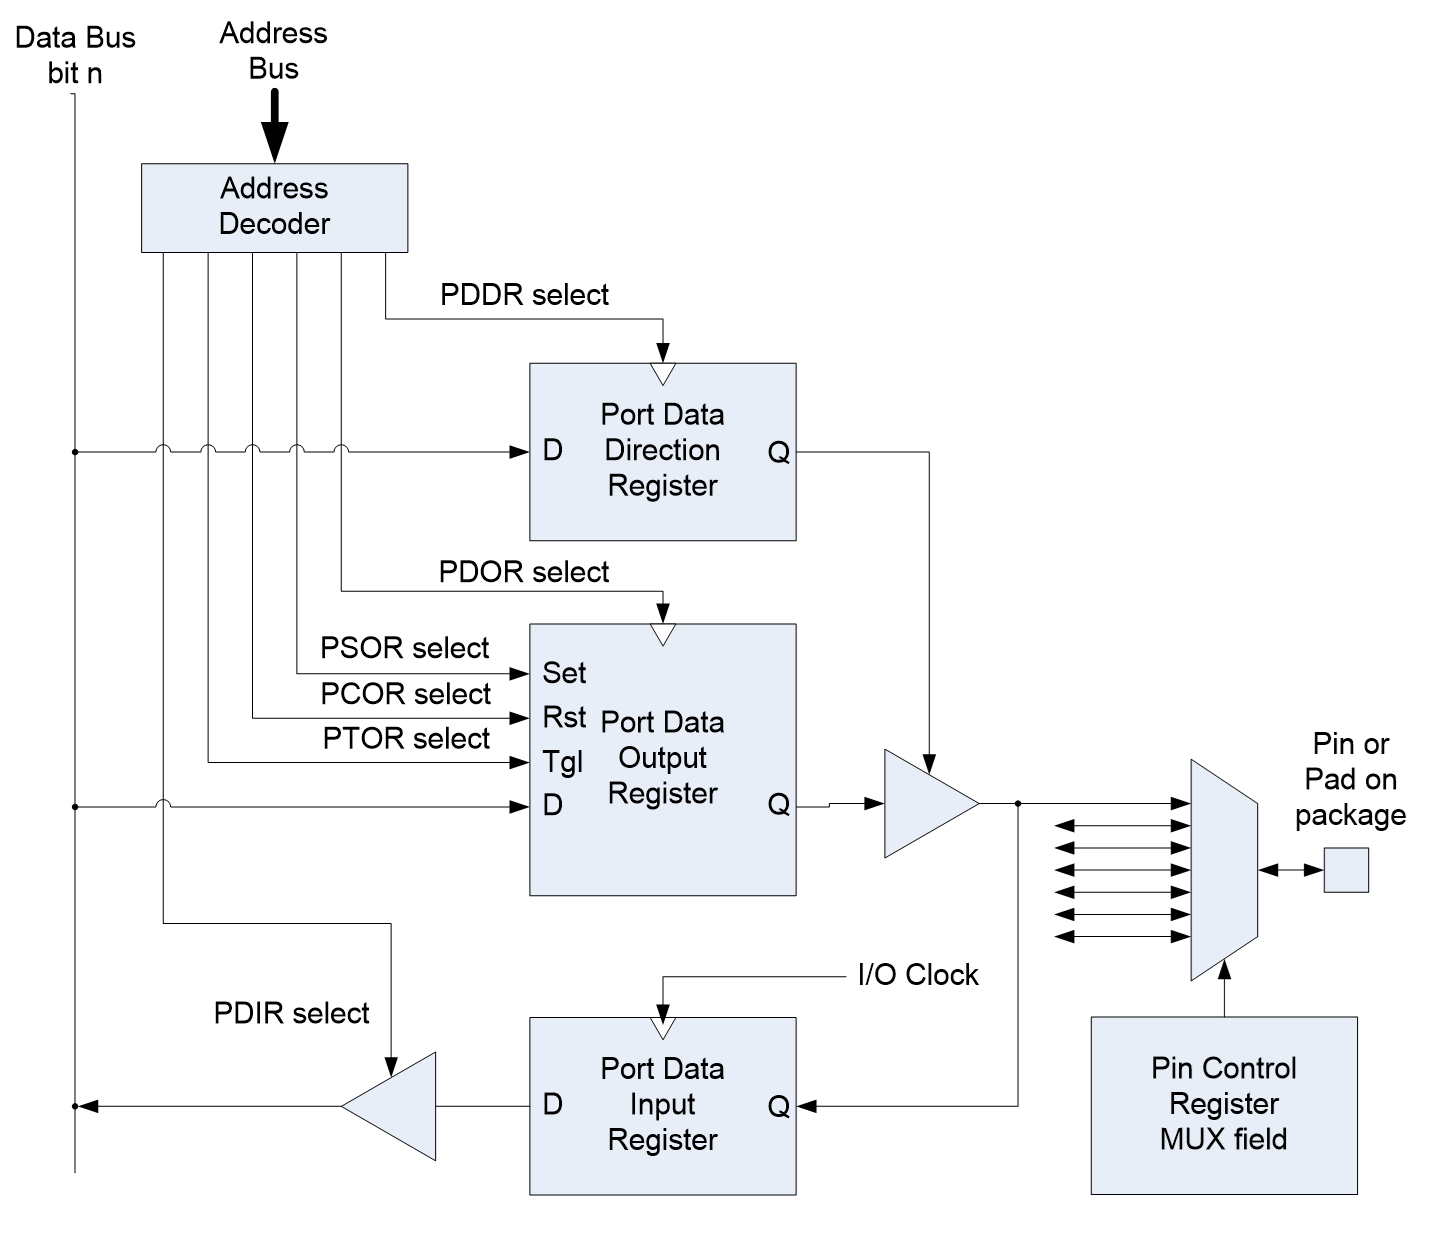
\includegraphics[scale=0.3]{07_GPIOCircuit}
	\end{figure}
\end{frame}
%%%%%%%%%%%%%%%%% FRAME %%%%%%%%%%%%%%%%%%%%%%%%%%
\begin{frame}
	\frametitle{Conectar una senal del GPIO al pin}
	\begin{figure}
		\centering
		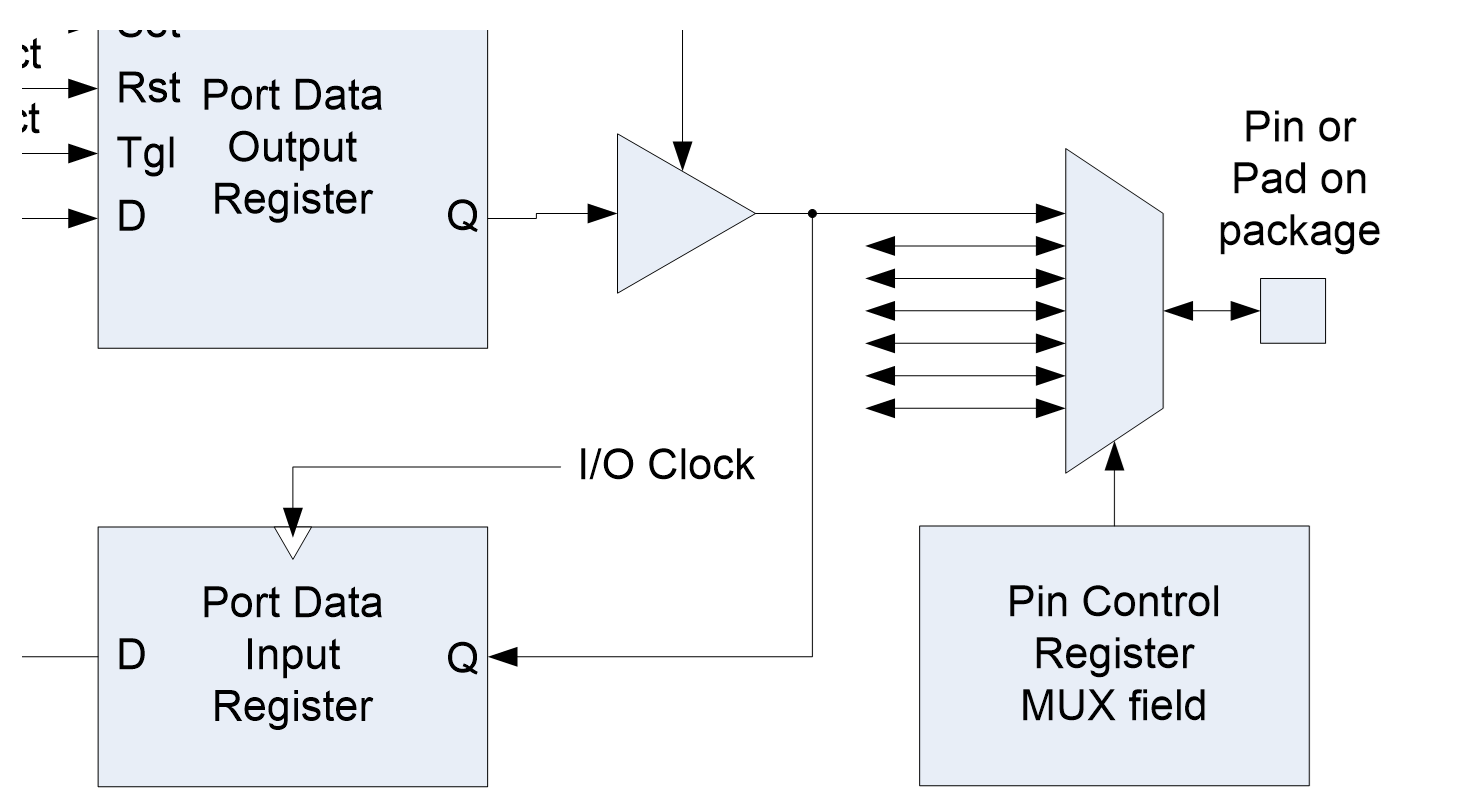
\includegraphics[scale=0.3]{08_MuxCircuit}
	\end{figure}
	\begin{itemize}
		\item Se utiliza un multiplexador para incrementar la configurabilidad del sistema y sus capacidades. 
		\item Cada pin configurable tiene un registro de control de pin, PCR (Pin Control Register)
	\end{itemize}
\end{frame}
%%%%%%%%%%%%%%%%% FRAME %%%%%%%%%%%%%%%%%%%%%%%%%%
\begin{frame}
	\frametitle{Registro de control de pin PCRn}
	\begin{figure}
		\centering
		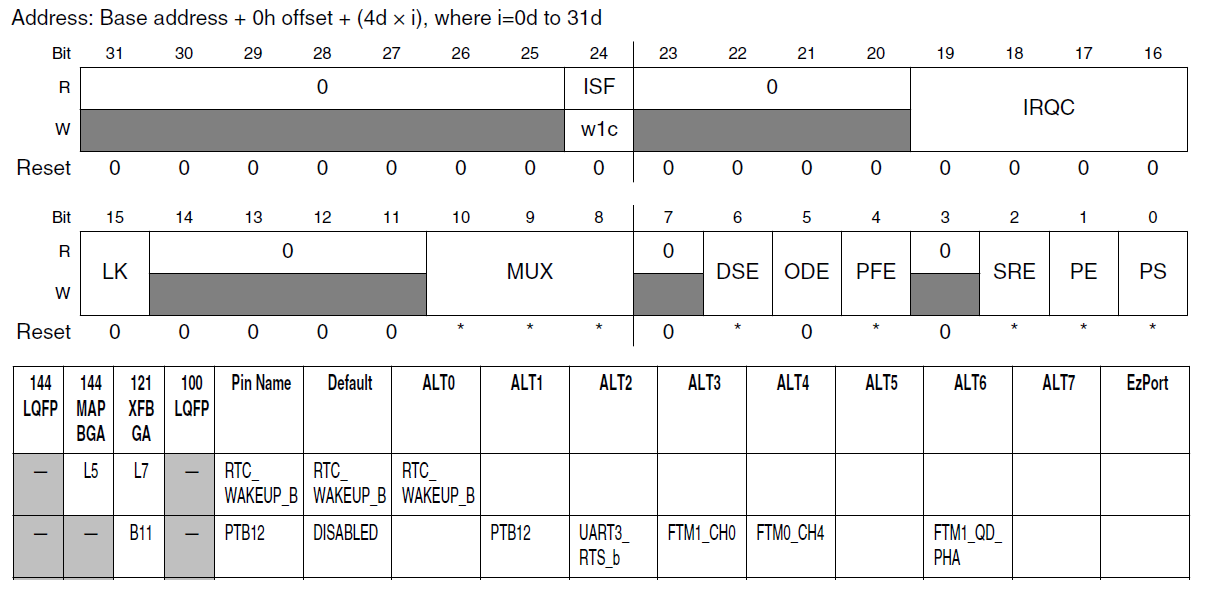
\includegraphics[scale=0.4]{09_PCR}
	\end{figure}
	\begin{columns}
		\column{0.5\linewidth}
		El campo del MUX define las conexiones internas de la señal.
		\column{0.5\linewidth}
		\begin{scriptsize}
			\begin{tabular}{ cc } 
				\hline
				\textbf{MUX (bit 10-8)} & \textbf{Configuración}  \\ 
				\hline
				000 & Pin deshabilitado  \\ 
				001 & ALT 1 - GPIO \\ 
				010 & ALT 2 \\ 
				011 & ALT 3 \\ 
				100 & ALT 4 \\ 
				101 & ALT 5 \\ 
				110 & ALT 6 \\ 
				111 & ALT 7 \\ 
				\hline
			\end{tabular}
		\end{scriptsize}
	\end{columns}
\end{frame}
%%%%%%%%%%%%%%%%% FRAME %%%%%%%%%%%%%%%%%%%%%%%%%%
\begin{frame}
	\frametitle{Registros control GPIO}
	\begin{figure}
		\centering
		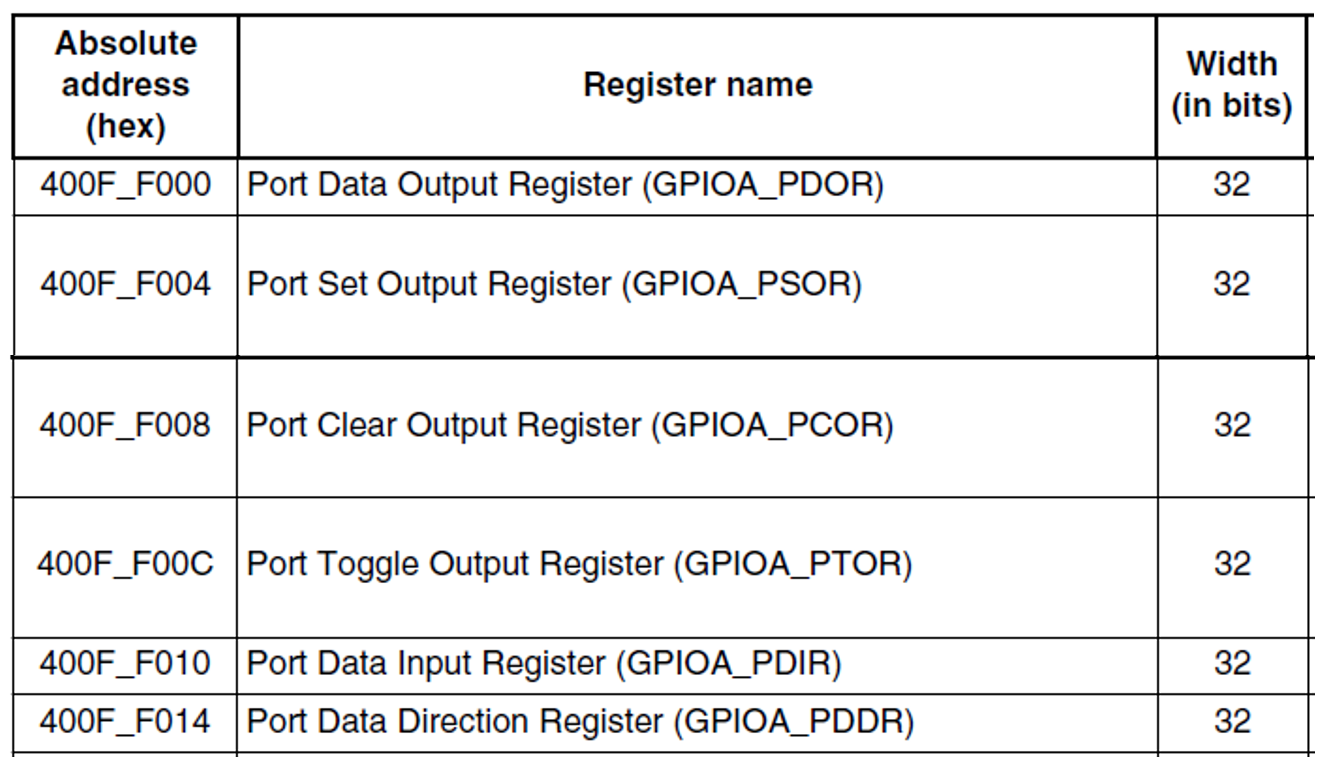
\includegraphics[scale=0.4]{10_RegistrosControlGPIO}
	\end{figure}
	\begin{itemize}
		\item Un conjunto de registro de control por puerto.
		\item Cada bit en un registro de control corresponde a un bit del puerto. 
	\end{itemize}
\end{frame}
%%%%%%%%%%%%%%%%% FRAME %%%%%%%%%%%%%%%%%%%%%%%%%%
\begin{frame}
	\frametitle{PDDR - Port Data Direction Register}
	\begin{columns}
		\column{0.4\linewidth}
		\begin{itemize}
			\item Cada bit puede ser configurado de manera independiente.
			\item Entrada: 0
			\item Salida: 1
			\item Un reset limpia el puerto y lo pone en cero. 
		\end{itemize}
		
		\column{0.6\linewidth}
		\begin{figure}
			\centering
			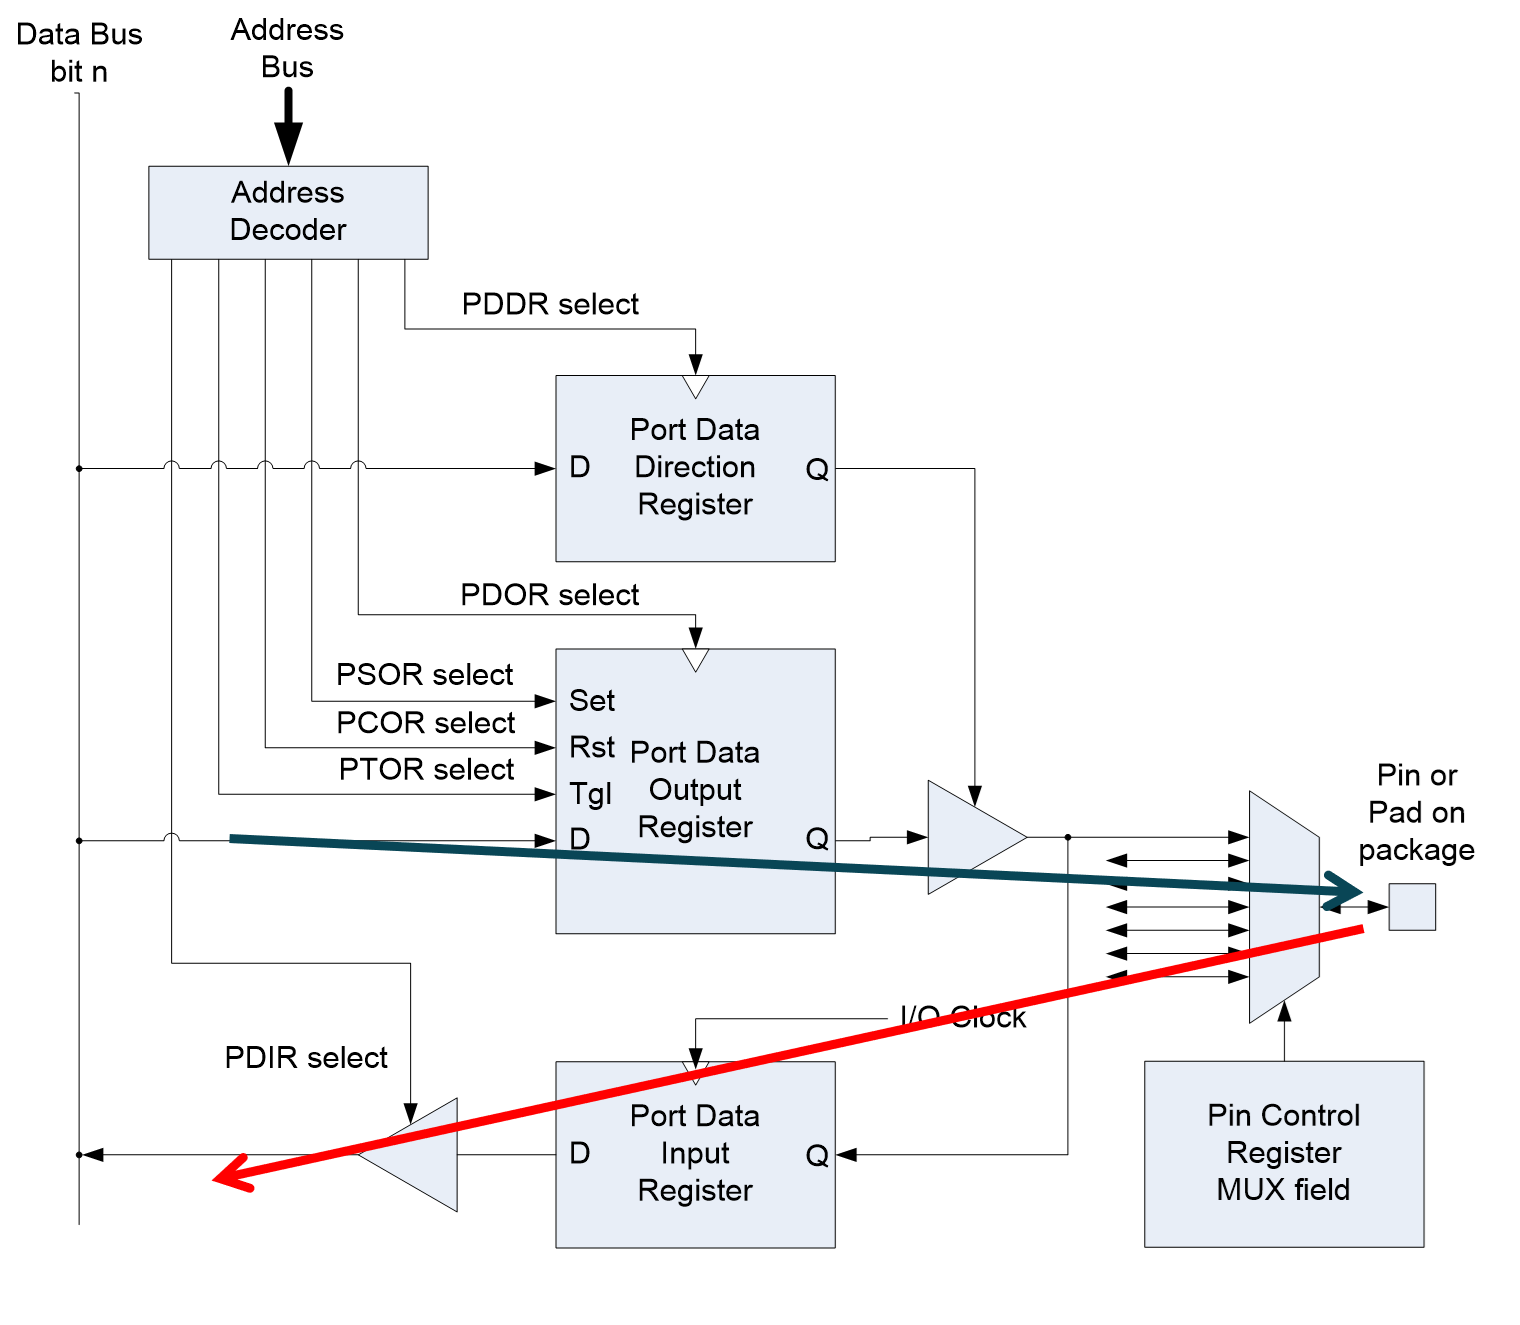
\includegraphics[scale=0.3]{11_PDDR}
		\end{figure}
	\end{columns}
\end{frame}
%%%%%%%%%%%%%%%%% FRAME %%%%%%%%%%%%%%%%%%%%%%%%%%
\begin{frame}
	\frametitle{Escribiendo un puerto}
	\begin{columns}
		\column{0.4\linewidth}
		\begin{itemize}
			\item Directo: escriba el valor en el PDOR
			\item Toggle: escriba un uno 1 en PTOR
			\item Clear (a 0): escriba un 1 en PCOR
			\item Set (a 1): escriba un 1 en PSOR 
		\end{itemize}
		
		\column{0.6\linewidth}
		\begin{figure}
			\centering
			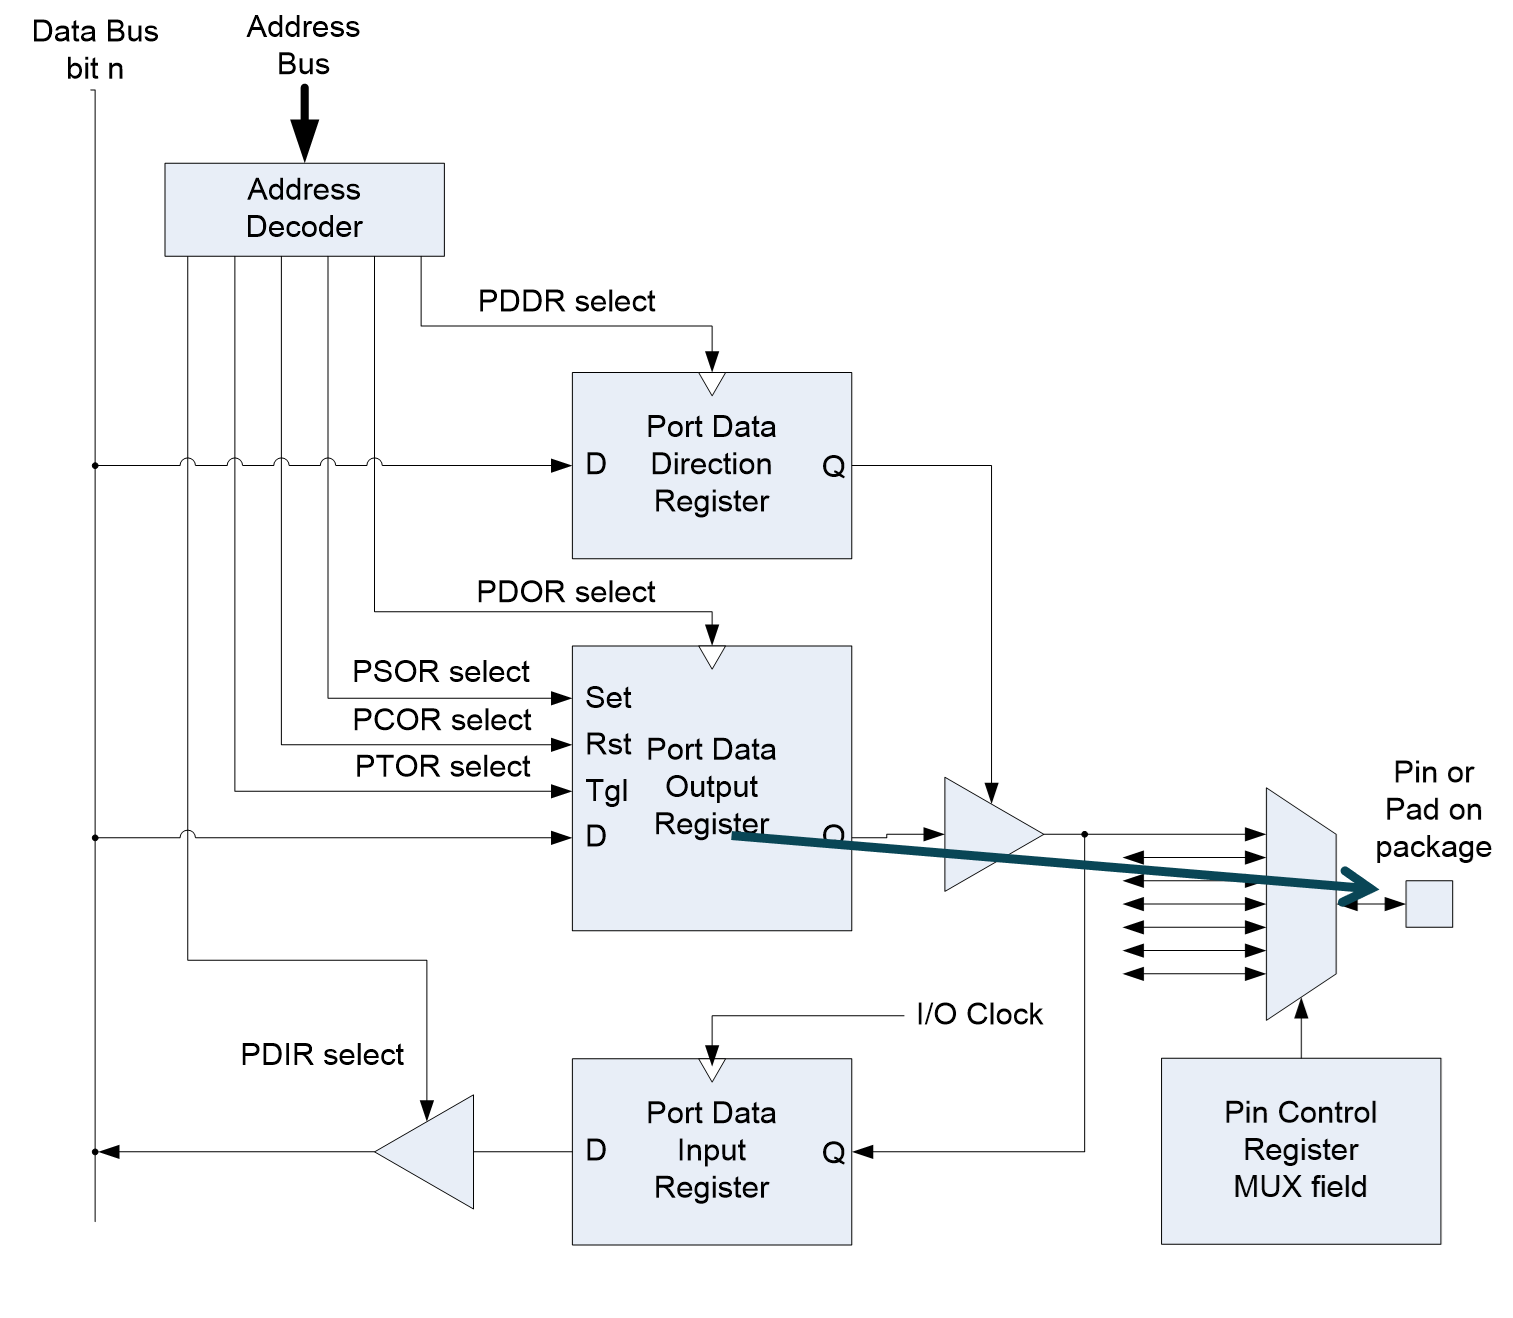
\includegraphics[scale=0.3]{12_WritingGPIO}
		\end{figure}
	\end{columns}
\end{frame}
%%%%%%%%%%%%%%%%% FRAME %%%%%%%%%%%%%%%%%%%%%%%%%%
\begin{frame}
	\frametitle{Leyendo un puerto}
	\begin{columns}
		\column{0.4\linewidth}
		\begin{itemize}
			\item Leerlo desde el PDIR
			\item El bit mantiene el valor de lectura realizado.  
		\end{itemize}
		
		\column{0.6\linewidth}
		\begin{figure}
			\centering
			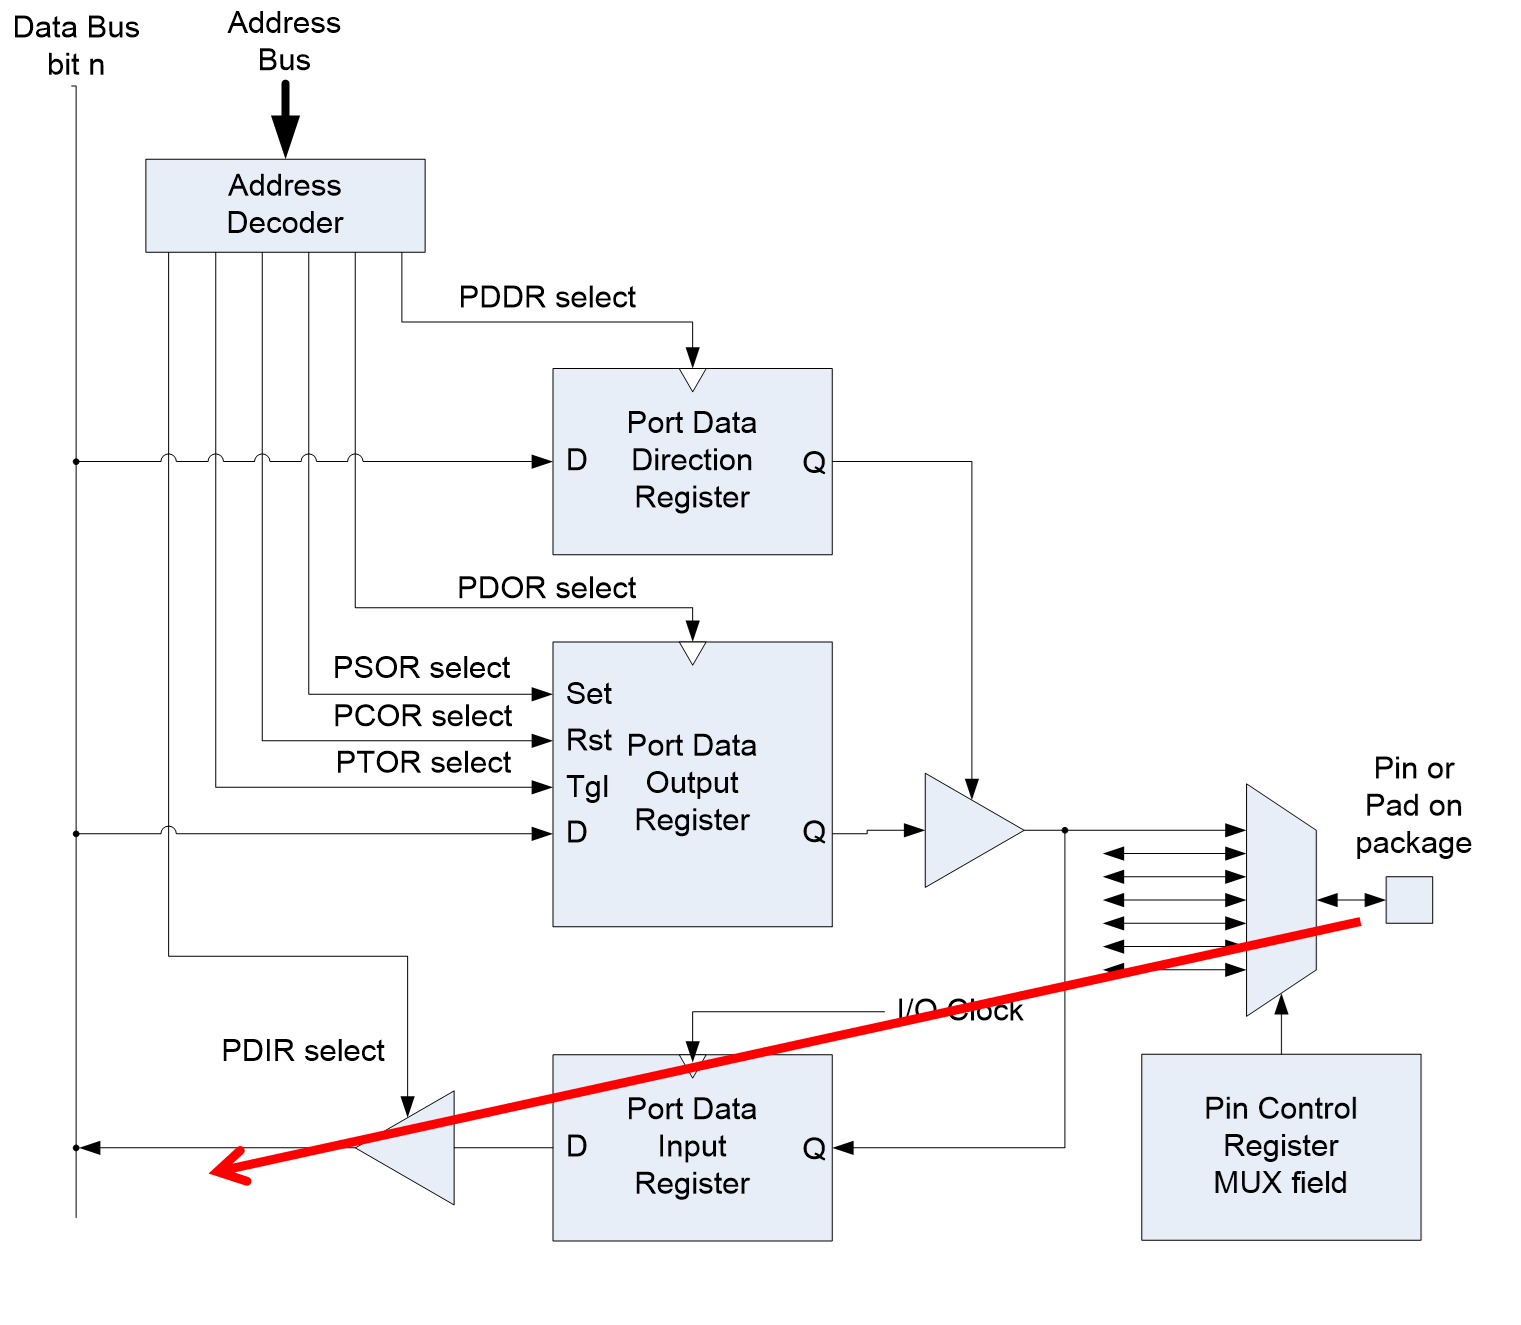
\includegraphics[scale=0.3]{13_ReadingGPIO}
		\end{figure}
	\end{columns}
\end{frame}
%%%%%%%%%%%%%%%%% FRAME %%%%%%%%%%%%%%%%%%%%%%%%%%
\begin{frame}[fragile]
	\frametitle{Como configurar en software?}
	Pseudocódigo
	\begin{lstlisting}[style=CStyle]
		// Make PTB21 and PTB22 outputs
		set bits 21 and 22 of GPIOB_PDDR 
		// Make PTA4 input
		clear bit 4 of GPIOA_PDDR
		// Initialize the output data values: LED 1 off, LED 2 on
		clear bit 21, set bit 22 of GPIOB_PDOR
		// read switch, light LED accordingly
		do forever {
			if bit 4 of GPIOA_PDIR is 1 { // switch is not pressed, so light LED 2
				set bit 22 of GPIOB_PDOR
				clear bit 21 of GPIOB_PDOR
			} else {			    // switch is pressed, so light LED 1
				set bit 21 of GPIOB_PDOR
				clear bit 22 of GPIOB_PDOR
			}
		}
	\end{lstlisting}
\end{frame}
%%%%%%%%%%%%%%%%% FRAME %%%%%%%%%%%%%%%%%%%%%%%%%%
\begin{frame}
	\frametitle{Estilo de codificacion y acceso a bits}
	\begin{itemize}
		\item Es facil cometer errores poniendo binarios o hexadecimales
		\begin{itemize}
			\item Para prender el bit 13 y 19 se usaria 0000 0000 0000 1000 0010 0000 0000 0000 or 0x00082000 
		\end{itemize}
		\item Use el valor literal para desplazar los bits
		\begin{itemize}
			\item[] n = (1UL $<<$ 19) $\mid$ (1UL $<<$ 13);
		\end{itemize}
		\item Realice macros para los pines
		\begin{itemize}
			\item[] \#define GREEN\_LED\_POS (19)
			\item[]	\#define YELLOW\_LED\_POS (13)
			\item[] n = (1UL $<<$ GREEN\_LED\_POS) $\mid$ (1UL $<<$ YELLOW\_LED\_POS);
		\end{itemize}
		\item Cree macros para el desplazamiento
		\begin{itemize}
			\item[] \#define MASK(x) (1UL $<<$ (x))
			\item[]	n = MASK(GREEN\_LED\_POS) $\mid$ MASK(YELLOW\_LED\_POS);
		\end{itemize}
	\end{itemize}
\end{frame}
%%%%%%%%%%%%%%%%% FRAME %%%%%%%%%%%%%%%%%%%%%%%%%%
\begin{frame}
	\frametitle{Usando las máscaras}
	\begin{itemize}
		\item Sobrescribir todo el registro con el valor de la máscara. 
		\begin{itemize}
			\item[] n = MASK(foo);
		\end{itemize}
		\item Poner 1 en n todos los valores que correspondan con 1 en la máscara, sin modificar los otros. 
		\begin{itemize}
			\item[] n $\mid$= MASK(foo);
		\end{itemize}
		\item Poner 0 en n todos los valores que correspondan con 1 en la máscara, sin modificar los otros. 
		\begin{itemize}
			\item[] n \&= $\sim$MASK(foo);
		\end{itemize}
		\item Nos ayudamos de CMSIS para acceder a los puertos. Analizar la hoja de datos la estructura GPIO. En donde PTx se define como un puntero a dicha estructura. 
	\end{itemize}
\end{frame}
%%%%%%%%%%%%%%%%% FRAME %%%%%%%%%%%%%%%%%%%%%%%%%%
\begin{frame}[fragile]
	\frametitle{Ejemplo codificado}
	\begin{multicols}{2}
		\begin{lstlisting}[style=CStyle]
#include "MK64F12.h"

#define LED1_POS (21)
#define LED2_POS (22)
#define SW1_POS (4)
#define MASK(x) (1UL << (x))
#define MASK(x) (1UL << (x))

int main(void){
	// Enable Clock Port A and B
	SIM->SCGC5 |= SIM_SCGC5_PORTA_MASK | SIM_SCGC5_PORTB_MASK;
	
	// Make 3 pins GPIO
	PORTB->PCR[LED1_POS] &= ~PORT_PCR_MUX_MASK;
	PORTB->PCR[LED1_POS] |= PORT_PCR_MUX(1);
	PORTB->PCR[LED2_POS] &= ~PORT_PCR_MUX_MASK;
	PORTB->PCR[LED2_POS] |= PORT_PCR_MUX(1);
	PORTA->PCR[SW1_POS] &= ~PORT_PCR_MUX_MASK;
	PORTA->PCR[SW1_POS] |= PORT_PCR_MUX(1);
	
	
	PTB->PDDR |= MASK(LED1_POS) | MASK(LED2_POS); // set bits to outputs
	PTA->PDDR &= ~MASK(SW1_POS); // clear switch bit to input
	
	PTB->PDOR = MASK(LED2_POS);  // turn on LED1, turn off LED2
	
	while (1) {
		if (PTA->PDIR & MASK(SW1_POS)) { // switch is not pressed, so light LED 2
			PTB->PDOR = MASK(LED2_POS);
		} else {	                   // switch is pressed, so light LED 1
			PTB->PDOR = MASK(LED1_POS);
		}
	}
}
		\end{lstlisting}
	\end{multicols}	
\end{frame}
%%%%%%%%%%%%%%%%% FRAME %%%%%%%%%%%%%%%%%%%%%%%%%%
\begin{frame}
	\frametitle{Chequeo para el uso de pines}
	\begin{columns}
		\column{0.5\linewidth}
		\begin{figure}
			\centering
			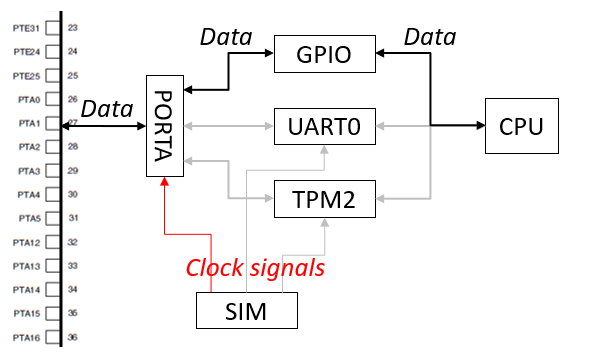
\includegraphics[scale=0.5]{14_ChequeoPines}
		\end{figure}
		
		
		\column{0.5\linewidth}
		\begin{itemize}
			\item Módulo SIM le habilita el clock a
			\begin{itemize}
				\item Módulo de puertos.
				\item Algunos periféricos (puede o no ser puerto)
			\end{itemize}
			\item Configurar el pin de control MUX
			\item Configurar el periférico
			\item Configurar la interrupción del sistema si es del caso. 
		\end{itemize}
	\end{columns}
\end{frame}
%%%%%%%%%%%%%%%%% FRAME %%%%%%%%%%%%%%%%%%%%%%%%%%
\begin{frame}
	\frametitle{Lógica para el clock}
	\begin{center}
		\begin{tabular}{ cc } 
			\hline
			\textbf{Bit} & \textbf{Puerto}  \\ 
			\hline
			13 & PORTE  \\ 
			12 & PORTD \\ 
			11 & PORTC \\ 
			10 & PORTB \\ 
			9  & PORTA \\  
			\hline
		\end{tabular}
	\end{center}
	\begin{itemize}
		\item Se necesita habilitar el clock al módulo GPIO.
		\item Por defecto vienen desactualizados para conservar energía.
		\item Si se escribe a un GPIO desactivado, sale error por hardware. 
		\item El registro de control SIM\_SCGC5 contiene el clock de los GPIO
		\item Habilitar el clock al puerto A.
		\begin{itemize}
			\item[] SIM-$>$SCGC5 $\mid=$ (1UL $<<$  9);
		\end{itemize}
		\item Utilizando las definiciones del Header. 
		\begin{itemize}
			\item[] SIM-$>$SCGC5 $\mid=$ SIM\_SCGC5\_PORTA\_MASK;
		\end{itemize}
	\end{itemize}
	
\end{frame}
%%%%%%%%%%%%%%%%% FRAME %%%%%%%%%%%%%%%%%%%%%%%%%%
\begin{frame}
	\frametitle{Soporte del CMSIS para el PCR}
	\begin{itemize}
		\item El devive.h define la estructura PORT\_type con los campos incluyendo PCR como un vector de 32 enteros. 
	\end{itemize}
	\begin{figure}
		\centering
		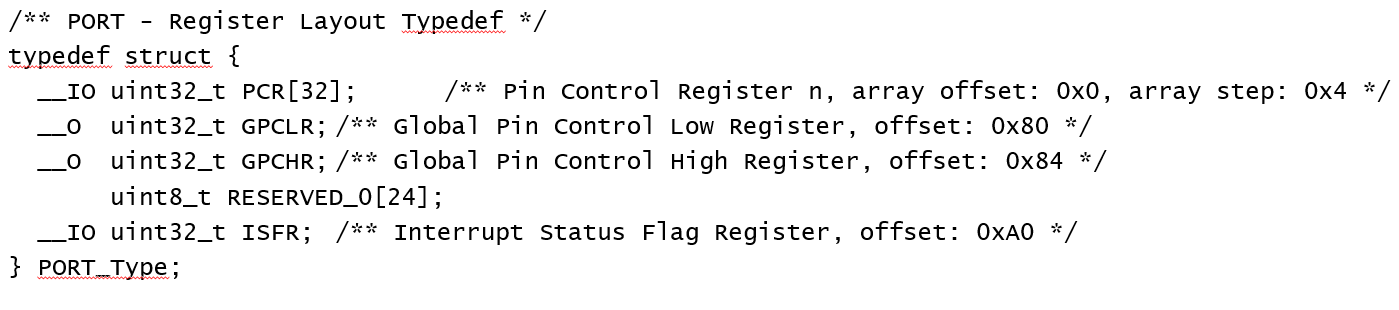
\includegraphics[scale=0.4]{15_PCRStructure}
	\end{figure}
\end{frame}
%%%%%%%%%%%%%%%%% FRAME %%%%%%%%%%%%%%%%%%%%%%%%%%
\begin{frame}
	\frametitle{Soporte del CMSIS para el PCR}
	\begin{figure}
		\centering
		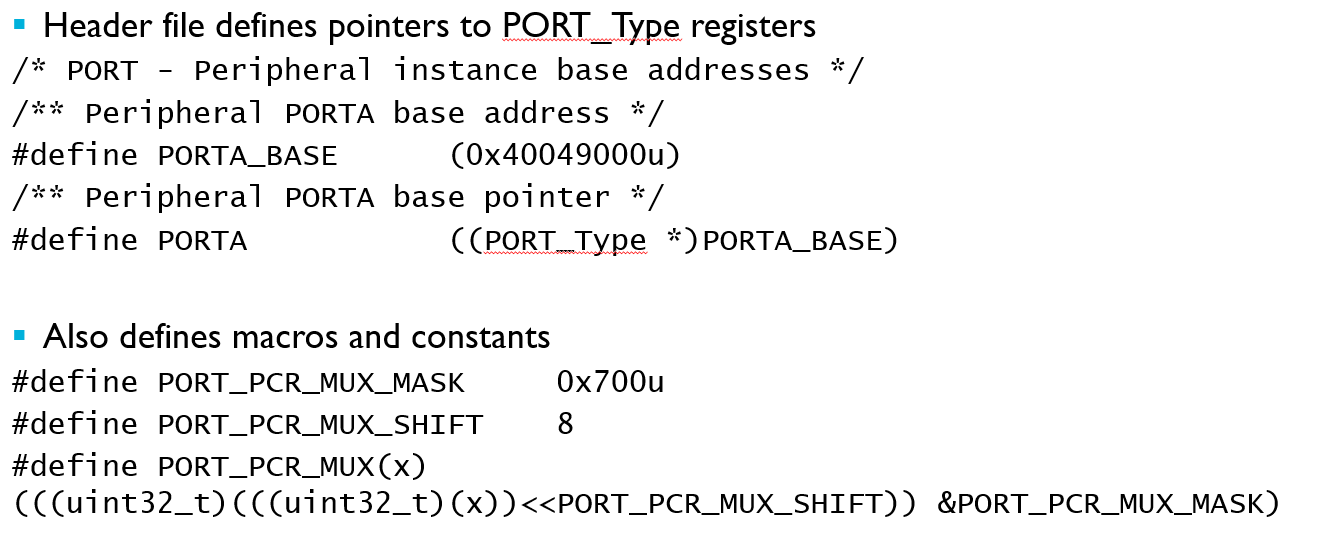
\includegraphics[scale=0.4]{16_MaskPCR}
	\end{figure}
\end{frame}

%%%%%%%%%%%%%%%%% FRAME %%%%%%%%%%%%%%%%%%%%%%%%%%
\begin{frame}
	\frametitle{Ejemplo LCD}
	\begin{columns}
		\column{0.5\linewidth}
		\begin{itemize}
			\item Pantalla de cristal liquido
			\item Hay de diferentes tamaños: 16x2, 16x4, etc.
			\item Puede comunicarse con 4 o 8-bits
			\item[] 
			\begin{small}
				\begin{center}
					\begin{tabular}{ c c c }
						\hline
						\textbf{Pin} & \textbf{Símbolo} & \textbf{Descripción} \\ 
						\hline
						1 & Vss & Tierra \\  
						2 & Vcc & Fuente  \\
						3 & Vee & Contraste \\
						4 & RS & 0 com, 1 dat \\
						5 & RW & 0 escri, 1 lect \\
						6 & E & enable \\
						7-14 & D0-D7 & Bus de datos \\
						15 & A & Ánodo \\
						16 & K & Cátodo \\
						\hline  
					\end{tabular}
				\end{center}
			\end{small}
		\end{itemize}
		\column{0.5\linewidth}
		\begin{figure}
			\centering
			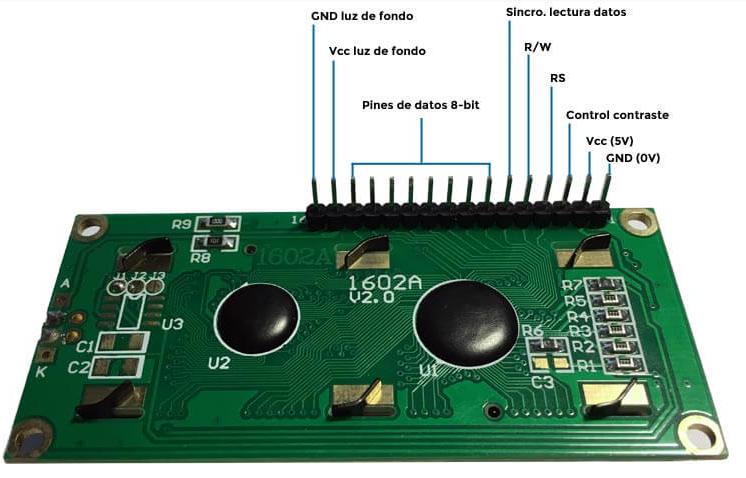
\includegraphics[scale=0.37]{17_LCD}
		\end{figure}
	\end{columns}
\end{frame}
%%%%%%%%%%%%%%%%% FRAME %%%%%%%%%%%%%%%%%%%%%%%%%%
\begin{frame}
	\frametitle{Ejemplo LCD - Comando y conexiones}
	\begin{columns}
		\column{0.5\linewidth}	
		\begin{small}
			\begin{center}
				\begin{tabular}{ c c  }
					\hline
					\textbf{Codigo (Hex)} & \textbf{Comando}   \\ 
					\hline
					1 & Limpia el display  \\  
					2 & Retorna cursor al home \\
					6 & Incrementa el cursor \\
					F & Display on, y cursor parpadea \\
					80 & Inicia cursor en primera linea \\
					C0 & Cursor en segunda linea\\
					28 & 2 lineas, 5x7 car, 4-bit \\
					\hline  
				\end{tabular}
			\end{center}
		\end{small}

		\column{0.5\linewidth}
		\begin{figure}
			\centering
			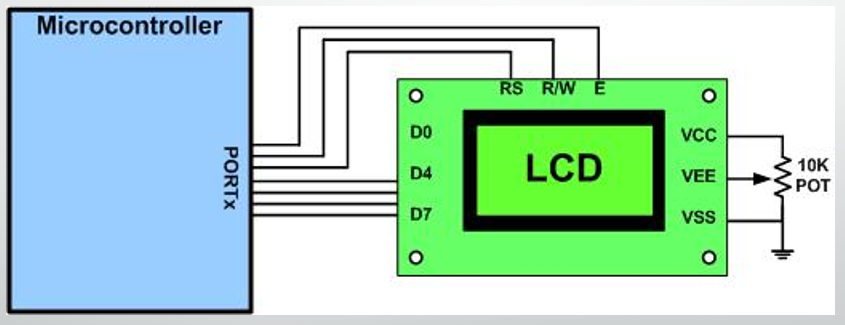
\includegraphics[scale=0.37]{18_LCDConex}
		\end{figure}
	\end{columns}

	\begin{itemize}
		\item Inicializar el LCD antes de usarlo.
		\item Crear funciones para envió de datos y envió de comandos.
		\item Respetar diagramas de tiempo. 
	\end{itemize}
\end{frame}

%%%%%%%%%%%%%%%%% FRAME %%%%%%%%%%%%%%%%%%%%%%%%%%
\begin{frame}
	\frametitle{Ejemplo LCD - Diagrama de tiempo e inicialización}
	\begin{columns}
		\column{0.5\linewidth}	
		\begin{figure}
			\centering
			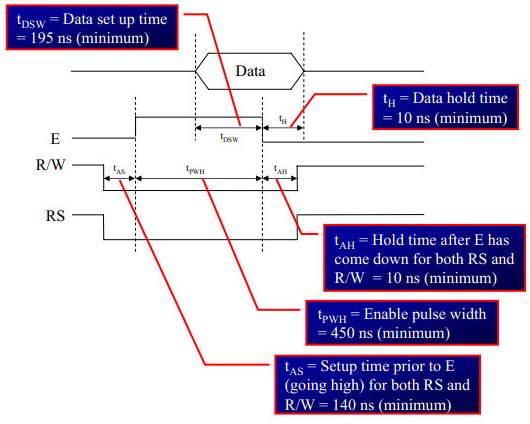
\includegraphics[scale=0.4]{19_TimingDiagramLCD}
		\end{figure}
		
		\column{0.5\linewidth}
		\begin{figure}
			\centering
			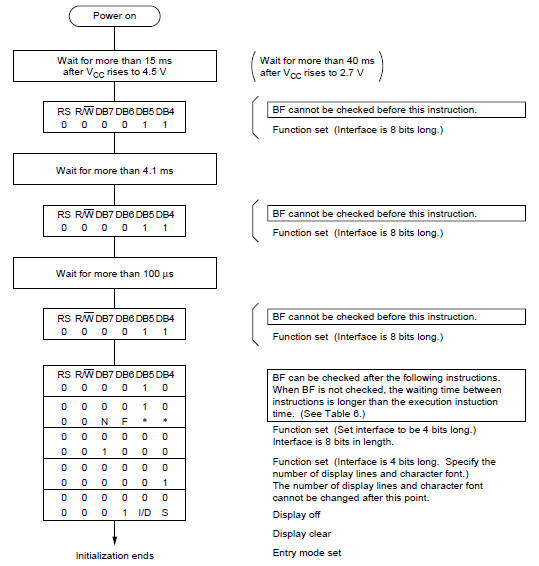
\includegraphics[scale=0.45]{20_Init4Bit}
		\end{figure}
	\end{columns}
\end{frame}

%%%%%%%%%%%%%%%%% FRAME %%%%%%%%%%%%%%%%%%%%%%%%%%
\begin{frame}[fragile]
	\frametitle{Ejemplo LCD - Creando la Libreria}
	\begin{itemize}
		\item Inicializar GPIO a utilizar
		\item Crear una función de retraso en ms. Aprox.
		\item Crear una función que dado un char me active los cuatros pines seleccionados. 
		\item Crear la funcion de envio de datos.
		\item Crear la funcion de envio de comandos. 
		\item Crear funciones auxiliares tales como: escribir una cadena, limpiar la pantalla, poner el cursor en una posición dada.
	\end{itemize}

	\begin{lstlisting}[style=CStyle]
		#define D7	16	/* PTC16 */
		#define D6	17	/* PTC17 */
		#define D5	9	/* PTB9 */
		#define D4	1	/* PTA1 */
		#define RS	23	/* PTB23 */
		#define EN	2	/* PTA2 */
		#define MASK(x) (1UL << (x))
	\end{lstlisting}
	El pin RW se pone a tierra ya que siempre se esta escribiendo la pantalla. 
\end{frame}

%%%%%%%%%%%%%%%%% FRAME %%%%%%%%%%%%%%%%%%%%%%%%%%
\begin{frame}[fragile]
	\frametitle{Ejemplo LCD - Software}
	\begin{itemize}
		\item Creando la función que pone el dato en el bus.
		\begin{lstlisting}[style=CStyle]
			void LcdDataBus(unsigned char Data){
				if(Data & 1)
				PTA->PSOR|= MASK(D4);
				else
				PTA->PCOR|= MASK(D4);
				if(Data & 2)
				PTB->PSOR|= MASK(D5);
				else
				PTB->PCOR|= MASK(D5);
				if(Data & 4)
				PTC->PSOR|= MASK(D6);
				else
				PTC->PCOR|= MASK(D6);
				if(Data & 8)
				PTC->PSOR|= MASK(D7);
				else
				PTC->PCOR|= MASK(D7);
			}
		\end{lstlisting}
	\end{itemize}	
\end{frame}
%%%%%%%%%%%%%%%%% FRAME %%%%%%%%%%%%%%%%%%%%%%%%%%
\begin{frame}[fragile]
	\frametitle{Ejemplo LCD - Software}
	\begin{itemize}
		\item Creando la función para escribir comandos.
		\begin{lstlisting}[style=CStyle]
void Lcd_CmdWrite(unsigned char cmd)
{
	LcdDataBus((cmd>>4) & 0x0F);     //Send higher nibble
	PTB->PCOR = MASK(RS);	   	   // Send LOW pulse on RS pin for selecting Command register
	PTA->PSOR = MASK(EN);	  	  // Generate a Low-to-High pulse on EN pin
	delayMs(4);
	PTA->PCOR = MASK(EN);	  	  // Generate a High-to-low pulse on EN pin
	
	
	delayMs(4);
	
	LcdDataBus(cmd & 0x0F); //Send Lower nibble
	PTB->PCOR = MASK(RS);	   	   // Send LOW pulse on RS pin for selecting Command register
	PTA->PSOR = MASK(EN);	  	  // Generate a Low-to-High pulse on EN pin
	delayMs(4);
	PTA->PCOR = MASK(EN);	  	  // Generate a High-to-low pulse on EN pin
	
	delayMs(5);
}
		\end{lstlisting}
	\end{itemize}	
\end{frame}
%%%%%%%%%%%%%%%%% FRAME %%%%%%%%%%%%%%%%%%%%%%%%%%
\begin{frame}[fragile]
	\frametitle{Ejemplo LCD - Software}
	\begin{itemize}
		\item Creando la función para inicializar el LCD.
		\begin{lstlisting}[style=CStyle]
    delayMs(30);                /* initialization sequence */
	Lcd_CmdWrite(0x33);          /* init */
	Lcd_CmdWrite(0x32);          /* init */
	
	Lcd_CmdWrite(0x28);          /* set 4-bit data, 2-line, 5x7 font */
	Lcd_CmdWrite(0x0C);          /* move cursor right */
	Lcd_CmdWrite(0x01);          /* clear screen, move cursor to home */
	Lcd_CmdWrite(0x06);          /* turn on display, cursor blinking */
		\end{lstlisting}
	\end{itemize}	
\end{frame}
%%%%%%%%%%%%%%%%% FRAME %%%%%%%%%%%%%%%%%%%%%%%%%%
\begin{frame}[fragile]
	\frametitle{Laboratorio 1 (15\%)}
	Hacer un programa en C que se pueda escribir cadenas en el LCD. 
	\begin{itemize}
		\item Recuerde inicializar el clock de cada puerto utilizado.
		\item Recuerde inicializar el registro de control PCR para los puertos utilizados como GPIO.
		\item Cree una función que envié datos al LCD.
		\item Cree una función que reciba una cadena y la muestre en el LCD.
		\item Cree una función que ponga el cursor en cualquier parte de la pantalla.
	\end{itemize}	
\end{frame}
%%%%%%%%%%%%%%%%% FRAME %%%%%%%%%%%%%%%%%%%%%%%%%%
\begin{frame}[fragile]
	\frametitle{Laboratorio - Opcional}
	Hacer un programa en C lea un teclado matricial de 4x4 o 5x5. 
	\begin{columns}
		\column{0.5\linewidth}
		\begin{figure}
			\centering
			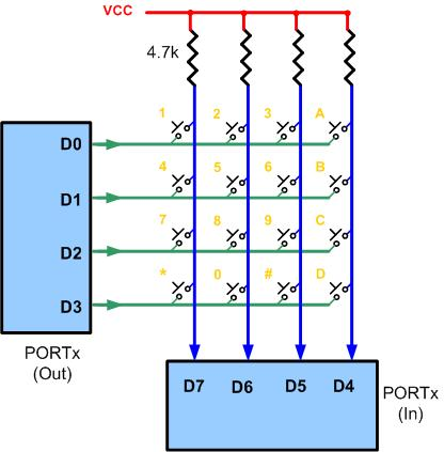
\includegraphics[scale=0.45]{21_Keyboard}
		\end{figure}
		\column{0.5\linewidth}
		\begin{figure}
			\centering
			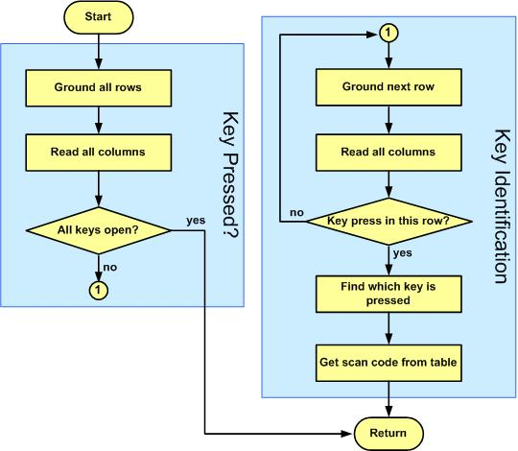
\includegraphics[scale=0.45]{22_KeyboardDF}
		\end{figure}
	\end{columns}	
\end{frame}
%%%%%%%%%%%%%%%%% FRAME %%%%%%%%%%%%%%%%%%%%%%%%%%
\frame{
\begin{center}
	\LARGE \textcolor{blue}{GENERAL PURPOSE INPUT-OUTPUT GPIO}
\end{center}

\begin{center}
	\LARGE \textcolor{blue}{GRACIAS}
\end{center}
}

%%%%%%%%%%%%%%%%%%%%%%%%%%%%%%%%%%%%%%%%%%%%%%%%%%%%%%%%%%%%%%%%%%%%%%%%%%%%%%%%%%%%%%%%%%%%%%%%%%%%%%%%%%%%%



\end{document}

